\section{Correspondence}

\begin{frame}{Recap: diepte meten}
\centerline{\begin{tikzpicture}[scale=0.75,cap=round]

    % let's define some key values
    \def\xc{-12}
    \def\xs{-3}
    \def\yimageplanes{1.25}
    \def\imageplaneshalfwidth{1.5}
    \def\xdistoffsetf{\imageplaneshalfwidth  + 0.5}
    \def\xdistoffsetZa{\imageplaneshalfwidth  - 0.25}
    \def\xdistoffsetZr{\imageplaneshalfwidth  - 1.25}
    \def\ydistoffsetxl{\yimageplanes + 0.125}
    \def\ydistoffsetxr{\ydistoffsetxl}
    \def\ydistoffsetb{0}
    \def\ydistoffsetinterx{\ydistoffsetb}
    \def\xobject{-6.5}
    \def\objectdepth{5.5}
    \def\referencedepth{3 + \objectdepth}
    \coordinate (pa) at (\xobject,\objectdepth);
    \coordinate (s) at (\xs,0);
    \coordinate (c) at (\xc,0);
    \coordinate (rayl2) at (\xc,0);
    \coordinate (ipll) at (\xc - \imageplaneshalfwidth, \yimageplanes);
    \coordinate (iplr) at (\xc + \imageplaneshalfwidth, \yimageplanes);


    % intersections of normals and reference plane
    \coordinate (rnrdi) at (\xs, \referencedepth);
    \coordinate (lnrdi) at (\xc, \referencedepth);
    % intersections of normals and object plane
    \coordinate (rnodi) at (\xs, \objectdepth);
    \coordinate (lnodi) at (\xc, \objectdepth);

    \coordinate (pr) at (intersection of s--pa and lnrdi--rnrdi);

    % intersection of c -- pr and object plane
    \coordinate (cprodi) at (intersection of c--pr and rnodi--lnodi);

    % pixel on image plane and expected pixel on image plane
    \coordinate (pixel) at (intersection of ipll--iplr and pa--c);
    \coordinate (epixel) at (intersection of ipll--iplr and pr--c);

    % Styles
    \tikzstyle{axes}=[]

    \begin{scope}[style=axes]
    \draw[->, thick] (0,0) -- (-15,0) node (xaxis) [below] {$x$};
    \draw[->, thick] (0,0) -- (0,10) node (zaxis) [above] {$z$};
    \draw[->, very thick] (0,0) -- (0.5,-0.625) node [below] {$y$};

    \end{scope}

    % point on object
    \draw [fill, red] (pa) circle (0.05) node [above right] {$p_a$};

    % point on reference plane
    \draw [fill, purple] (pr) circle (0.05) node [above right] {$p_r$};

    % left camera
    \draw [fill, blue] (-12,0) circle (0.05) node [below left] {$c$};
    % left image plane
    \draw[-, thick] (\xc - \imageplaneshalfwidth,\yimageplanes) -- 
        (\xc + \imageplaneshalfwidth, \yimageplanes);

    % right camera
    \draw [fill, blue] (-3,0) circle (0.05) node [below right] {$s$};

    % depth plane
    \draw[dashed, domain=-16:2] plot (\x, {\objectdepth});
     
    % Reference plane
    \draw[dashed, domain=-16:2] plot (\x, {\referencedepth});
    % p_r

    % image ray
    \draw[dotted] (pa)--(c);

    % projection ray
    \draw[dotted] (pr)--(s);
    
    % expected image ray
    \draw[dotted] (c)--(pr);

    % image points
    \draw[fill, orange] (pixel) circle (0.05) node [below right] {$x$};

    % focal length
    \draw[<->, thick, gray] (\xc - \xdistoffsetf,0) -- (\xc - \xdistoffsetf,\yimageplanes)
        node [midway, left, gray] {$f$};
    
    % Camera norms
    % left
    \draw[->] (c) -- (\xc, \referencedepth + 1);
    % perpendicular symbol
    \draw[thick] (\xc,0.15) -| (\xc-0.15, 0); 
    % right
    \draw[->] (s) -- (\xs, \referencedepth + 1);
    % perpendicular symbol
    \draw[thick] (\xs,0.15) -| (\xs +0.15, 0); 
    %(\xs,0)
    
    % actual depth
    \draw[<->, thick, gray] (\xc - \xdistoffsetZa, 0)
        -- (\xc - \xdistoffsetZa, \objectdepth)
        node [midway, left, gray] {$Z_{a}$};
    % reference depth
    \draw[<->, thick, gray] (\xc - \xdistoffsetZr, 0)
        -- (\xc - \xdistoffsetZr, \referencedepth)
        node [midway, left, gray] {$Z_{r}$};
    
    % camera distance
    \draw[<->, very thick, gray] (\xc,\ydistoffsetb) -- (\xs,\ydistoffsetb)
        node [midway, below, gray] {$b$};
    
    % point disparity over epipolar line
    \draw[<->, very thick, gray] (cprodi) -- (pa) node [midway, above, gray] {$d_o$};
    % point disparity over image plane
    \draw[<->, very thick, gray] (epixel) -- (pixel) node [midway, above, gray] {$d_i$};
    
\end{tikzpicture}
}
\begin{block}{Bepaal afstand $Z_a$}
{\small \begin{equation*} 
    \{ \frac{d_o}{b} = \frac{Z_r - Z_a}{Z_r}, \ \ \frac{d_i}{f} = \frac{d_o}{Z_a} \} \implies Z_a = \frac{Z_r}{d_i \frac{Z_r}{b f} + 1}
\end{equation*}
}
\end{block}
\end{frame}

\begin{frame}{Recap: diepte meten}
\centerline{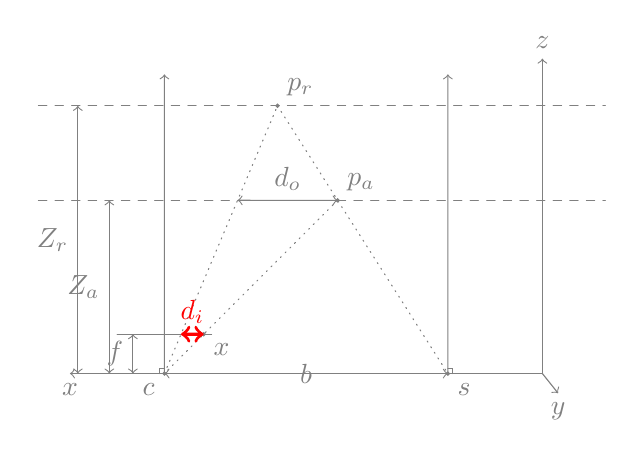
\begin{tikzpicture}[scale=0.40, cap=round]

    % let's define some key values
    \def\xc{-12}
    \def\xs{-3}
    \def\yimageplanes{1.25}
    \def\imageplaneshalfwidth{1.5}
    \def\xdistoffsetf{\imageplaneshalfwidth  + 0.5}
    \def\xdistoffsetZa{\imageplaneshalfwidth  - 0.25}
    \def\xdistoffsetZr{\imageplaneshalfwidth  - 1.25}
    \def\ydistoffsetxl{\yimageplanes + 0.125}
    \def\ydistoffsetxr{\ydistoffsetxl}
    \def\ydistoffsetb{0}
    \def\ydistoffsetinterx{\ydistoffsetb}
    \def\xobject{-6.5}
    \def\objectdepth{5.5}
    \def\referencedepth{3 + \objectdepth}
    \coordinate (pa) at (\xobject,\objectdepth);
    \coordinate (s) at (\xs,0);
    \coordinate (c) at (\xc,0);
    \coordinate (rayl2) at (\xc,0);
    \coordinate (ipll) at (\xc - \imageplaneshalfwidth, \yimageplanes);
    \coordinate (iplr) at (\xc + \imageplaneshalfwidth, \yimageplanes);


    % intersections of normals and reference plane
    \coordinate (rnrdi) at (\xs, \referencedepth);
    \coordinate (lnrdi) at (\xc, \referencedepth);
    % intersections of normals and object plane
    \coordinate (rnodi) at (\xs, \objectdepth);
    \coordinate (lnodi) at (\xc, \objectdepth);

    \coordinate (pr) at (intersection of s--pa and lnrdi--rnrdi);

    % intersection of c -- pr and object plane
    \coordinate (cprodi) at (intersection of c--pr and rnodi--lnodi);

    % pixel on image plane and expected pixel on image plane
    \coordinate (pixel) at (intersection of ipll--iplr and pa--c);
    \coordinate (epixel) at (intersection of ipll--iplr and pr--c);

    % Styles
    \tikzstyle{axes}=[]

    \begin{scope}[style=axes]
    \draw[->, gray] (0,0) -- (-15,0) node (xaxis) [below] {$x$};
    \draw[->, gray] (0,0) -- (0,10) node (zaxis) [above] {$z$};
    \draw[->, gray] (0,0) -- (0.5,-0.625) node [below] {$y$};

    \end{scope}

    % point on object
    \draw [fill, gray] (pa) circle (0.05) node [above right] {$p_a$};

    % point on reference plane
    \draw [fill, gray] (pr) circle (0.05) node [above right, gray] {$p_r$};

    % left camera
    \draw [fill, gray] (-12,0) circle (0.05) node [below left, gray] {$c$};
    % left image plane
    \draw[-, gray] (\xc - \imageplaneshalfwidth,\yimageplanes) -- 
        (\xc + \imageplaneshalfwidth, \yimageplanes);

    % right camera
    \draw [fill, gray] (-3,0) circle (0.05) node [below right, gray] {$s$};

    % depth plane
    \draw[dashed, gray, domain=-16:2] plot (\x, {\objectdepth});
     
    % Reference plane
    \draw[dashed, gray, domain=-16:2] plot (\x, {\referencedepth});
    % p_r

    % image ray
    \draw[dotted, gray] (pa)--(c);

    % projection ray
    \draw[dotted, gray] (pr)--(s);
    
    % expected image ray
    \draw[dotted, gray] (c)--(pr);

    % image points
    \draw[fill, gray] (pixel) circle (0.05) node [below right, gray] {$x$};

    % focal length
    \draw[<->, gray] (\xc - \xdistoffsetf,0) -- (\xc - \xdistoffsetf,\yimageplanes)
        node [midway, left, gray] {$f$};
    
    % Camera norms
    % left
    \draw[->, gray] (c) -- (\xc, \referencedepth + 1);
    % perpendicular symbol
    \draw[gray] (\xc,0.15) -| (\xc-0.15, 0); 
    % right
    \draw[->, gray] (s) -- (\xs, \referencedepth + 1);
    % perpendicular symbol
    \draw[gray] (\xs,0.15) -| (\xs +0.15, 0); 
    %(\xs,0)
    
    % actual depth
    \draw[<->, gray] (\xc - \xdistoffsetZa, 0)
        -- (\xc - \xdistoffsetZa, \objectdepth)
        node [midway, left, gray] {$Z_{a}$};
    % reference depth
    \draw[<->, gray] (\xc - \xdistoffsetZr, 0)
        -- (\xc - \xdistoffsetZr, \referencedepth)
        node [midway, left, gray] {$Z_{r}$};
    
    % camera distance
    \draw[<->, gray] (\xc,\ydistoffsetb) -- (\xs,\ydistoffsetb)
        node [midway, gray] {$b$};
    
    % point disparity over epipolar line
    \draw[<->, gray] (cprodi) -- (pa) node [midway, above, gray] {$d_o$};
    % point disparity over image plane
    \draw[<->, very thick, red] (epixel) -- (pixel) node [midway, above, red] {$d_i$};
    
\end{tikzpicture}
}
\begin{block}{Bepaal afstand $Z_a$}
{\small \begin{equation*} 
    \{ \frac{d_o}{b} = \frac{Z_r - Z_a}{Z_r}, \ \ \frac{d_i}{f} = \frac{d_o}{Z_a} \} \implies Z_a = \frac{Z_r}{d_i \frac{Z_r}{b f} + 1}
\end{equation*}
}
\end{block}
\end{frame}

\begin{frame}{Correspondence problem}
\centerline{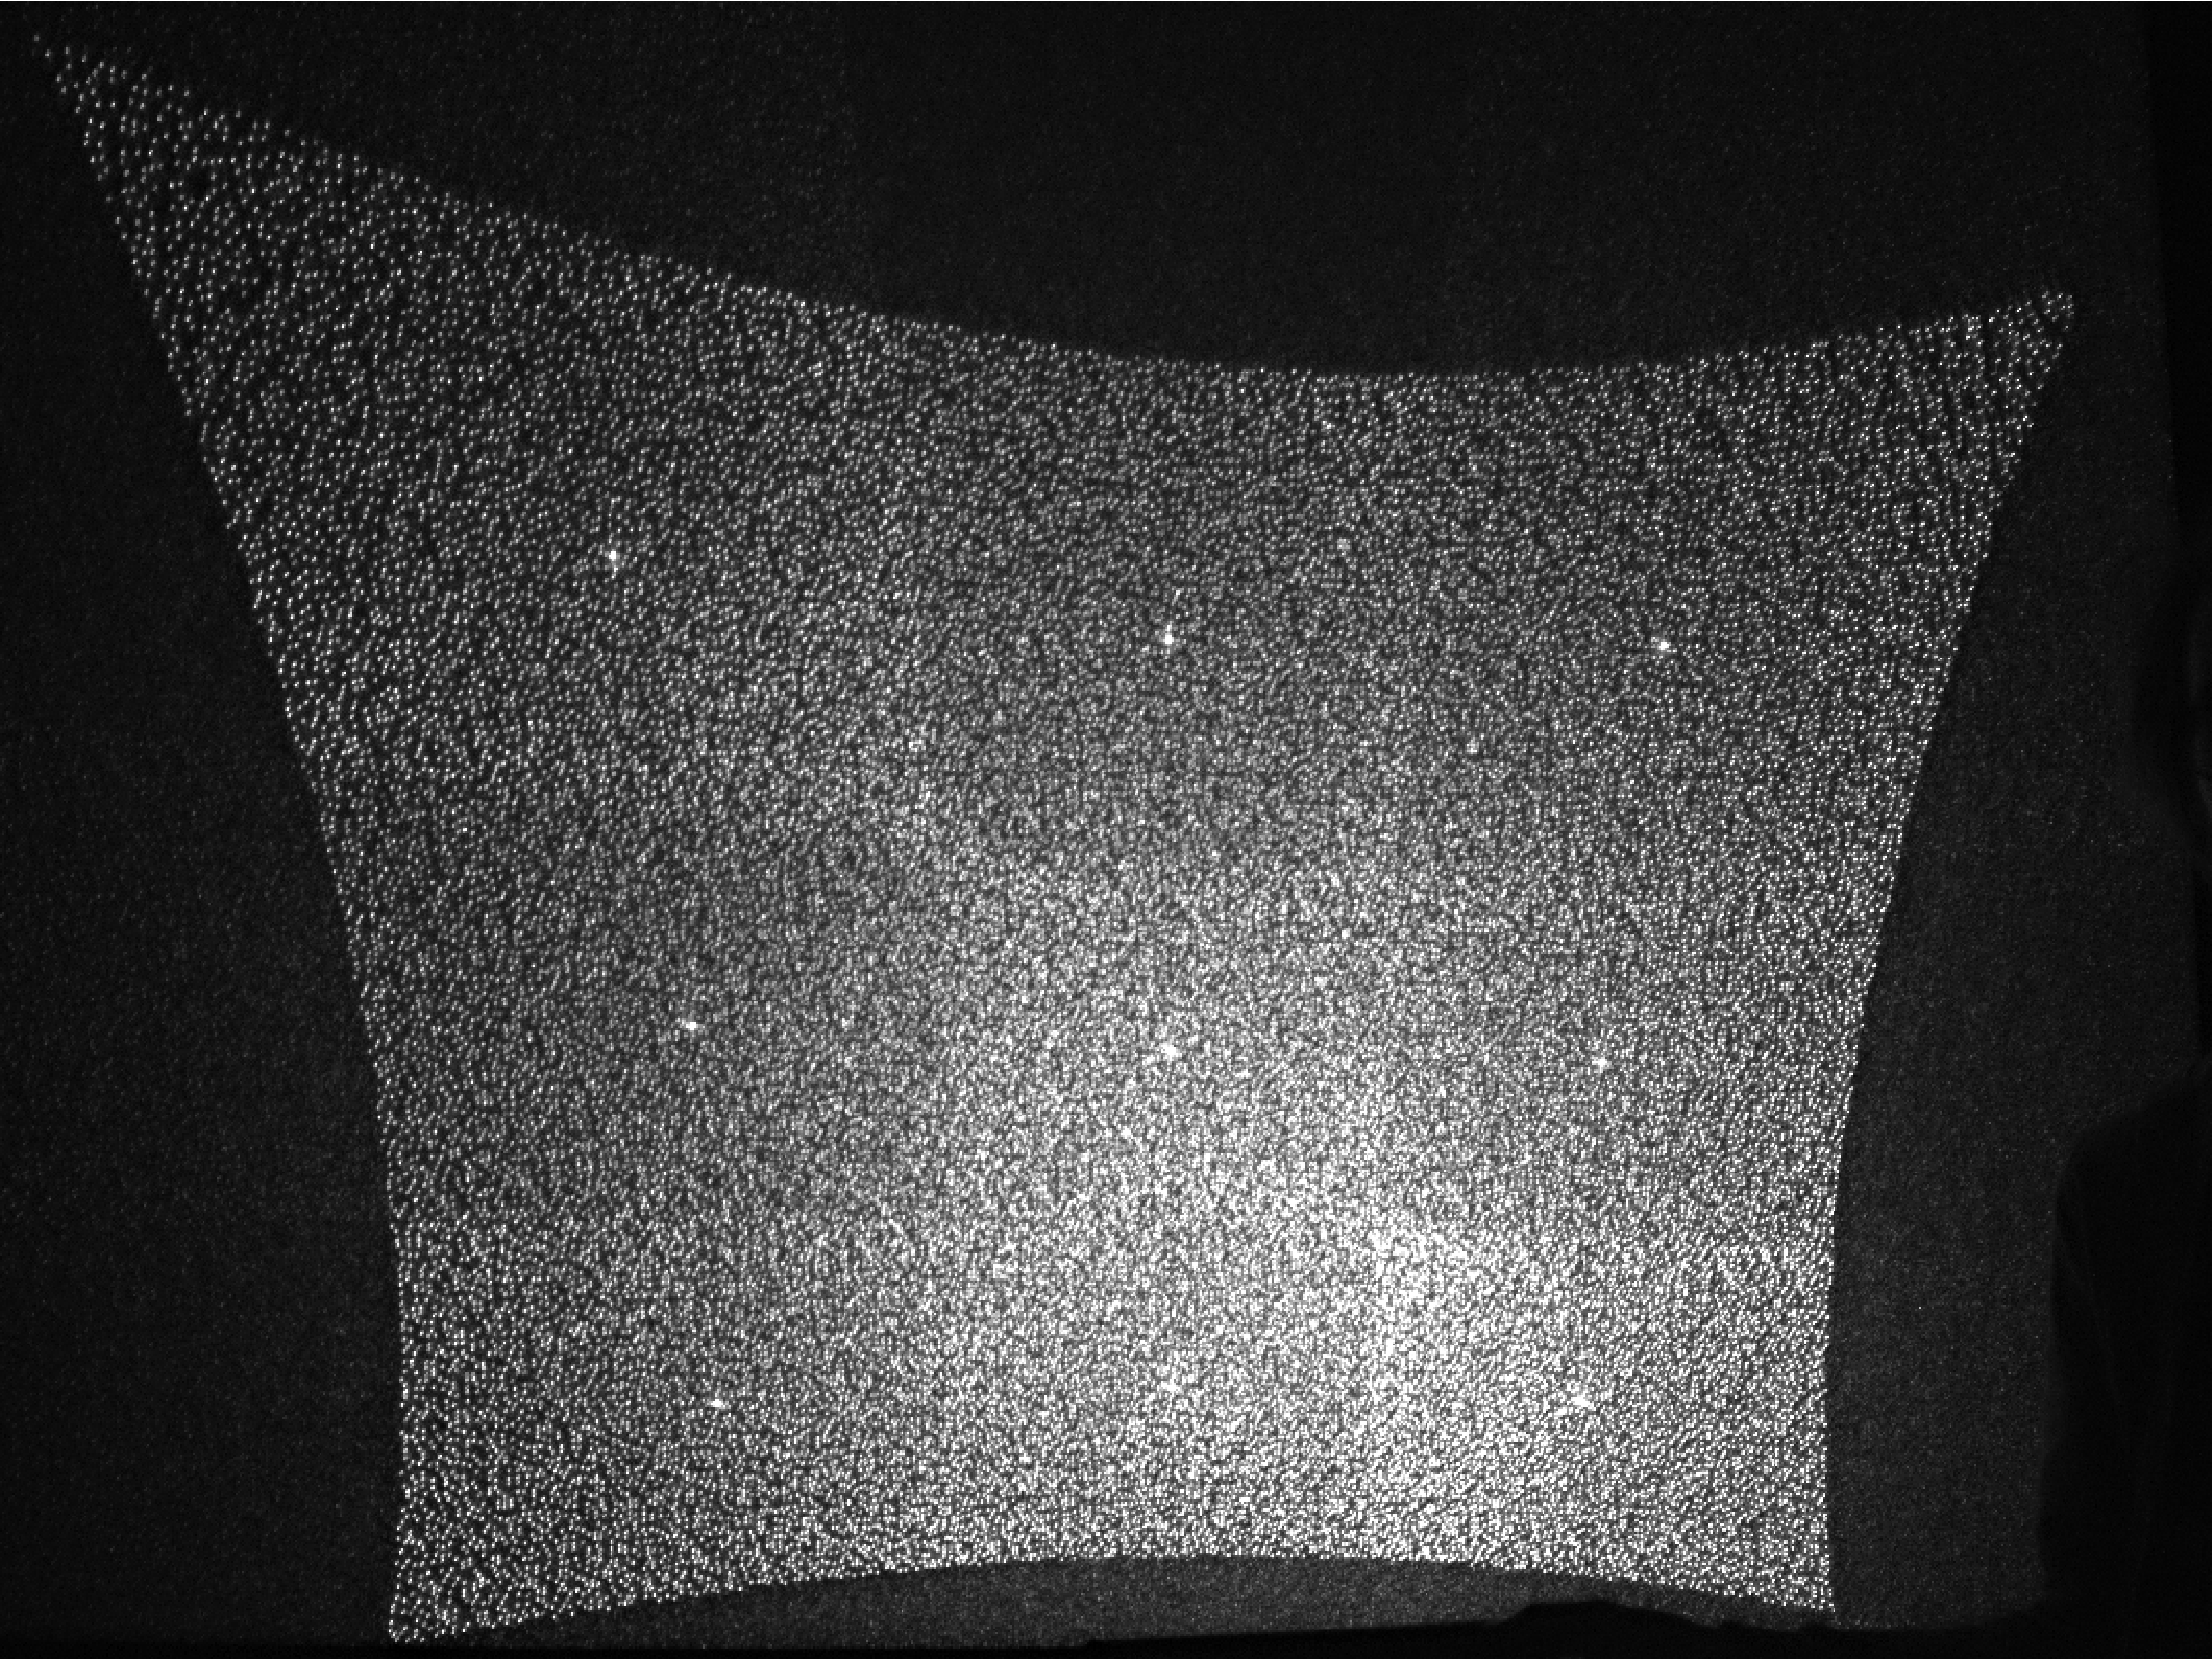
\includegraphics[scale=0.15]{images/whole_pattern}}
\begin{block}{Vier oplossingen}
\begin{enumerate}
\item Schaal invariante transformaties
\item Light coding
\item Schaal identificatie
\item Meerdere referentie beelden
\end{enumerate}
\end{block}
\end{frame}


\begin{frame}{Correspondence problem}
\centerline{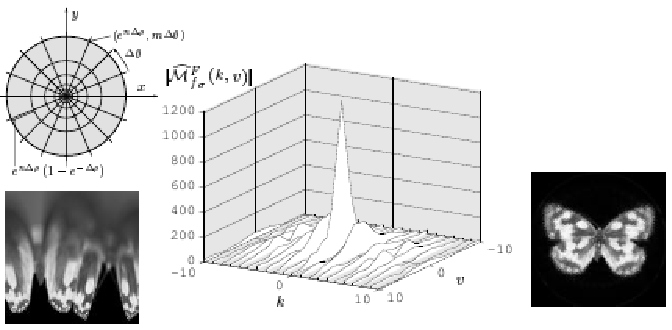
\includegraphics[scale=0.50]{images/mellin1}}
\begin{block}{Scale invariant transforms}
Mellin Transform
\end{block}
\pause
\begin{enumerate}
\item<+-> bewaar (Fourier-) Mellin representaties
\item<+-> voor elk punt
\begin{enumerate}[a.]
\item<+-> maak (F)M representaties van subregio's langs epipolaire lijn
\item<+-> correleer deze met bewaarde representaties
\item<+-> coordinaten referentie subregio met hoogste correlatie $\equiv x_r$
\end{enumerate}
\end{enumerate}
\end{frame}

\begin{frame}{Correspondence problem}
\centerline{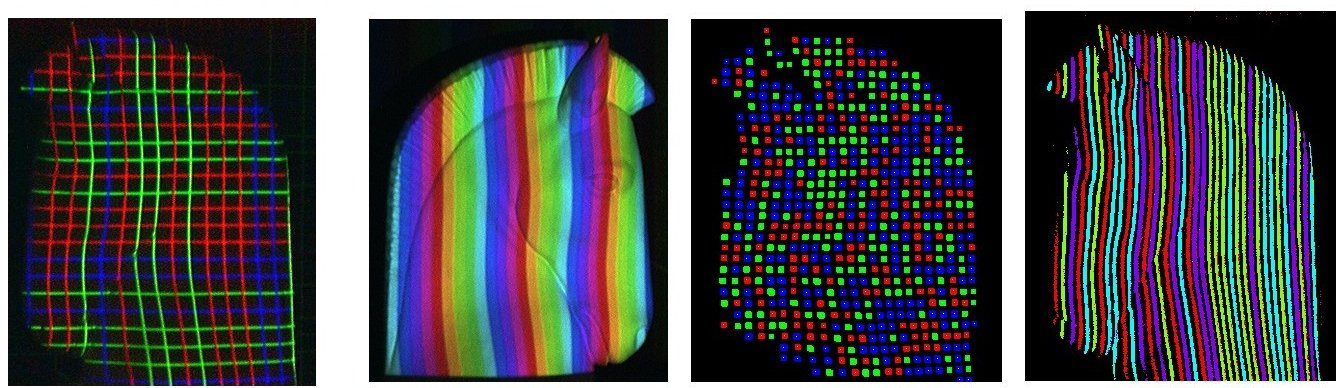
\includegraphics[scale=0.17]{structuredlight.jpg}}
\begin{block}{Light coding}
\begin{itemize}
\item specifiek voor actieve stereo triangulatie
\item patronen (e.g.\ de bruijn sequenties), kleuren, luminantie
\end{itemize}
\end{block}
\end{frame}

\begin{frame}{Correspondence problem}
\centerline{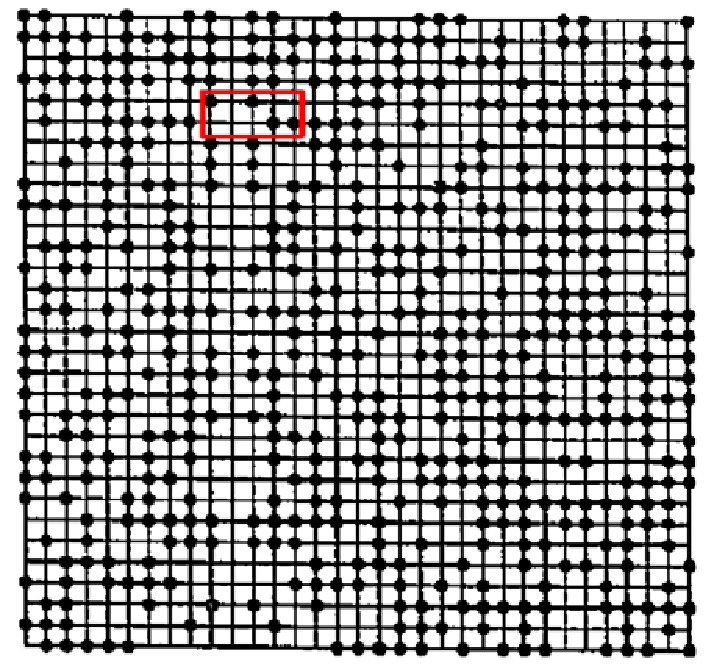
\includegraphics[scale=0.25]{images/prba}\, 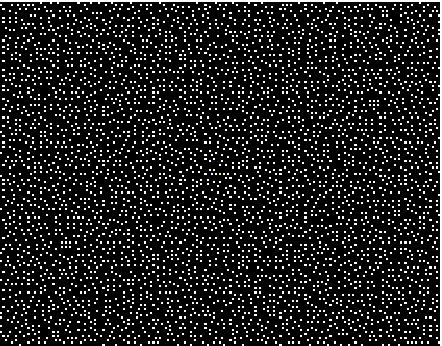
\includegraphics[scale=1, clip=true, viewport= 0 0 80 63]{kinect-pattern}   }
\begin{block}{Light coding}
Peudo Random Binary Array
\end{block}
\pause
\begin{enumerate}
\item<+-> stap een
\item<+-> voor elk punt
\begin{enumerate}[a.]
\item<+-> substap een
\item<+-> substap twee
\item<+-> substap drie
\end{enumerate}
\end{enumerate}
\end{frame}

\begin{frame}{Correspondence problem}
\centerline{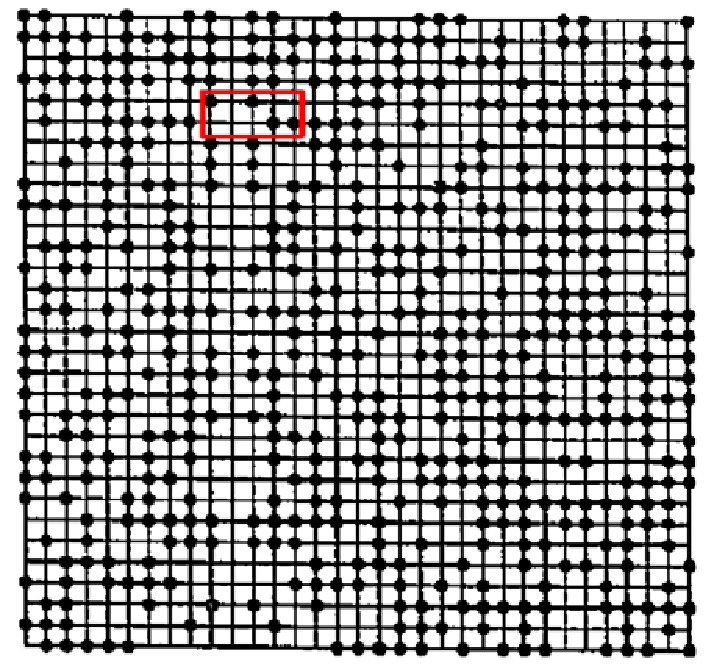
\includegraphics[scale=0.25]{images/prba}\, 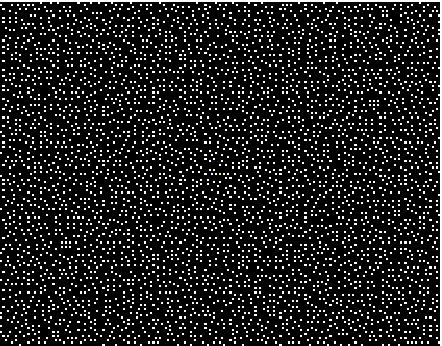
\includegraphics[scale=1, clip=true, viewport= 0 0 80 63]{kinect-pattern}   }
\begin{block}{Light coding}
Peudo Random Binary Array
\end{block}
\pause
\begin{enumerate}
\item<+-> stap een
\item<+-> voor elk punt
\begin{enumerate}[a.]
\item<+-> substap een
\item<+-> substap twee
\item<+-> substap drie
\end{enumerate}
\end{enumerate}
\end{frame}

\begin{frame}{Correspondence problem}
\centerline{\begin{tikzpicture}[scale=0.30, cap=round]

    % let's define some key values
    \def\xc{-12}
    \def\xs{-3}
    \coordinate (p) at (12,7);
    \coordinate (n1) at (13.75,8.5);
    \coordinate (n2) at (8,7.75);
    \coordinate (n3) at (13.25,2.5);
    \coordinate (nk) at (3,4);

    % Styles
    \tikzstyle{axes}=[]

    \begin{scope}[style=axes]
    \draw[->, gray] (0,0) -- (15,0) node (xaxis) [below] {$x$};
    \draw[->, gray] (0,0) -- (0,10) node (yaxis) [above] {$y$};

    \end{scope}

    % point
    \draw [fill, red] (p) circle (0.05) node [below right] {$x_i$};

    % neighbours
    \draw [fill] (n1) circle (0.05) ;
    \draw [fill] (n2) circle (0.05) ;
    \draw [fill] (n3) circle (0.05) ;
    \draw [fill] (nk) circle (0.05) ;


    % distances 
    \draw[<->, dotted, gray] (p) -- (n1) node [midway, left, gray] {$d_1$};
    \draw[<->, dotted, gray] (p) -- (n2) node [midway, left, gray] {$d_2$};
    \draw[<->, dotted, gray] (p) -- (n3) node [midway, left, gray] {$d_3$};
    \draw[<->, dotted, gray] (p) -- (nk) node [midway, left, gray] {$d_k$};
    
\end{tikzpicture}
}
\begin{block}{Schaal identificeren}
Gemiddelde afstanden
\end{block}
\pause
\begin{enumerate}
\item<+-> maak patroon waarvoor: 
\begin{enumerate}[a.]
\item<+-> $\overline{d_i}$ (zie plaatje), uniform over alle punten
\end{enumerate}
\item<+-> bewaar een referentie beeld en $R:\overline{d}\mapsto s$ ($s \equiv$ schaal)
\item<+-> voor elk punt
\begin{enumerate}[a.]
\item<+-> bereken $s$ m.b.v\ $R$
\item<+-> correleer langs horizontaal, met referentie beeld geschaald met $s$
\end{enumerate}
\end{enumerate}
\end{frame}

\begin{frame}{Correspondence problem}
\centerline{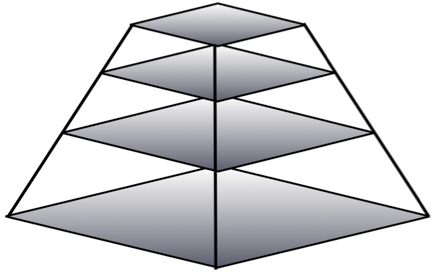
\includegraphics[scale=0.25]{images/pyramid}}
\begin{block}{Meerdere referentie beelden}
\begin{itemize}
\item geschikt voor parallelisatie
\item beperkte diepte
\end{itemize}
\end{block}
\pause
\begin{enumerate}
\item<+-> maak en bewaar aparte referentiebeelden voor reeks schalen
\item<+-> voor elk punt
\begin{enumerate}[a.]
\item<+-> correleer regios links en rechts met alle referentie beeld
\item<+-> referentie subregio met hoogste correlatie $\equiv x_r$
\end{enumerate}
\end{enumerate}
\end{frame}
